\documentclass[runningheads,a4paper]{llncs}

\usepackage{amssymb}
\setcounter{tocdepth}{3}
\usepackage{graphicx}
\usepackage{url}
\usepackage{color}
\usepackage{xspace}
\usepackage{float}

\newcommand{\comment}[1]{\marginpar{\scriptsize\textcolor{red}{#1}}}
%\definecolor{Orange}{rgb}{1,0.5,0}
\newcommand{\todo}[1]{\textbf{\textcolor{red}{[[#1]]}}}

\newcommand{\karma}{\textsc{Karma}\xspace}
\newcommand{\eg}{e.g.,\xspace}
\newcommand{\ie}{i.e.,\xspace}
\newcommand{\rtworml}{\textsc{r2rml}\xspace}
\newcommand{\sparql}{SPARQL\xspace}

\urldef{\mailsa}\path|{knoblock, pszekely, slepicka}@isi.edu|
\urldef{\mailsb}\path|{chengyey}@usc.edu|    
\newcommand{\keywords}[1]{\par\addvspace\baselineskip
\noindent\keywordname\enspace\ignorespaces#1}

\begin{document}
\mainmatter  % start of an individual contribution
% first the title is needed
\title{A Demonstration of Linked Data Source Discovery and Integration\protect\footnote{A video demonstration is available at http://youtu.be/sr-XDBKeNCY}}
% a short form should be given in case it is too long for the running head
\titlerunning{A Demonstration of Linked Data Discovery and Integration}
% the name(s) of the author(s) follow(s) next
%
\author{Jason Slepicka%
\and Chengye Yin\and Pedro Szekely\and Craig A. Knoblock}
%
\authorrunning{Slepicka et al.}
% (feature abused for this document to repeat the title also on left hand pages)
% the affiliations are given next; don't give your e-mail address
% unless you accept that it will be published
\institute{University of Southern California\\ 
Information Sciences Institute and Department of Computer Science, USA\\
\mailsa\\
\mailsb\\}
\maketitle
\begin{abstract}
%  1. The problem
The Linked Data cloud is an enormous repository of data, but it is difficult for users to find relevant data and integrate this data into their own datasets. 
%  2. Why the problem is a problem (why it's an interesting problem [SPJ])
Datasets in the Linked Data cloud are represented using ontologies, but lack accurate descriptions of the data they contain.
%  3. Startling sentence (what your solution achieves [SPJ])
We present an approach that leverages \rtworml mappings to describe the contents of datasets in order to find relevant data and integrate it with a user's own datasets.
%  4. Implication of startling sentence (what follows from your solution [SPJ])
Our demonstration shows how users can easily create \rtworml mappings for their datasets and then use these mappings to augment their datasets with data from the Linked Data cloud.
\end{abstract}

\section{Introduction} 
As users begin to semantically model their data and publish it as RDF to the linked data cloud, they should be able to take advantage of their work and discover linked data, so they can integrate it into their own datasets.  
For museum curators like those at the Amon Carter Museum of American Art, this means they could multiply their efforts by doing something as simple as filling in gaps like missing birth dates in their own data. 
They could also use linked data to verify their own data and identify inconsistencies between it and another museum's like the Smithsonian. \cite{knoblock12:eswc}

With the explosive growth in linked data lately, however, figuring out what data is actually available is difficult.
Fortunately, as the community aligns on standard source modeling techniques like R2RML for generating RDF, it is possible to reason about the entities and relationships users are trying to capture in their source models, especially if users within a domain use the same ontologies and share their source models.
By users sharing source models along with their data, we will demonstrate how users of Karma can discover such data and integrate it with their own.

\section{Datasets}
\begin{enumerate}
\item CSV file from a museum, containing 197 artists. %containing 2433 records of artworks by 

\item Linked Data created from the Smithsonian American Art Museum (SAAM) content management system including over 40,000 artworks and 8,000 artists. 
The Linked Data is accessible on a \sparql endpoint.
In previous work~\cite{Szekely:2013vq} ~\todo{cite saam-lod github} we mapped the SAAM dataset to the CIDOC CRM ontology~\cite{Doerr:2003:CCR:958671.958678}, producing a collection of \rtworml mapping files for 14 tables in the SAAM collection management system.
In the demonstration, we are using the SAAM LOD as a proxy for the Linked Data cloud to illustrate the vision of a Linked Data cloud populated with \rtworml models.

\item \rtworml repository containing \rtworml mappings downloaded from the Web and stored in a triple store accessible on a \sparql endpoint (separate from the Linked Data endpoint).
\karma provides a model manager component to manage the \rtworml repository (Fig~\ref{fig:model-manager-screenshot}).

\item owl:sameAs links between the artists in the first dataset and the artists from the Smithsonian dataset generated using LIMES \cite{ngomo2011limes}.

\end{enumerate}
\begin{figure*}[bth]
\begin{center}
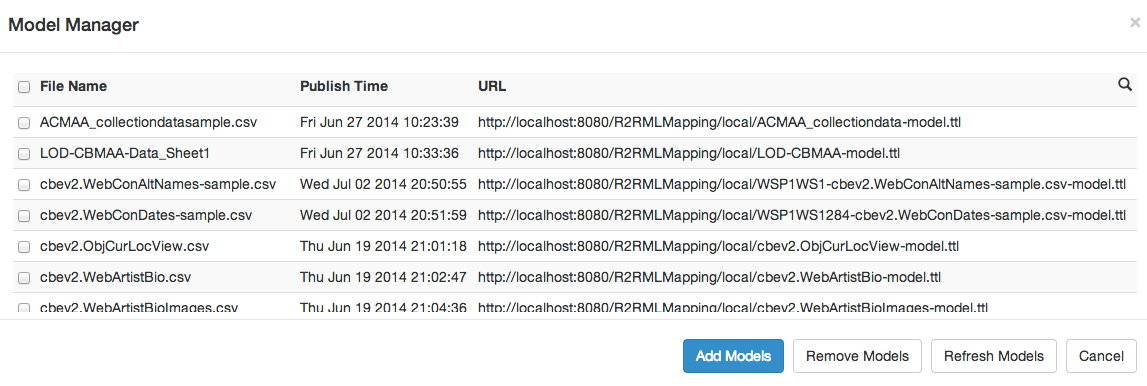
\includegraphics[width=4.8in]{images/3-model-manager.png}
\vspace{-3mm}
\caption{Screenshot of the model manager, showing the \rtworml mappings fetched from the GitHub repository where we shared the mappings for the SAAM dataset}
\vspace{-2mm}
\label{fig:model-manager-screenshot}
\end{center}
\vspace{-1.5em}
\end{figure*}
\section{Demonstration}
We will show how a user can interactively model an artist dataset, discover the Smithsonian's data for those artists, and then integrate the Smithsonian's data.  

\textbf{Step 1: Modeling a New Source.} 
The user begins by using Karma's existing capability to model the artists in the CSV file as crm:E21\_Person in an R2RML mapping shown in Figure~\ref{fig:simple-model-screenshot}.  
Karma can use this mapping to generate RDF. 
Karma can also compare it to the other mappings to discover new related sources that can be used to integrate with.
\begin{figure*}[b]
\centering
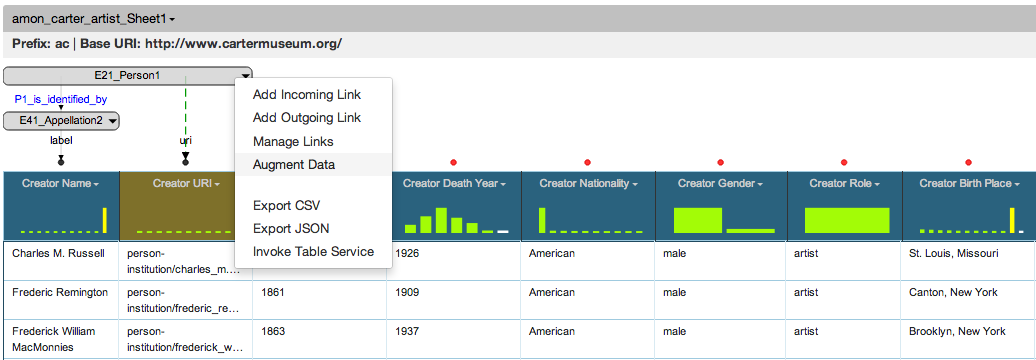
\includegraphics[width=4.8in]{images/4-simple-model.png}
\vspace{-20pt}
\caption{A Karma user creates an R2RML mapping for a CSV file of a museum's artists' biographical records and clicks 'Augment Data' to discover new data sources}
\vspace{-21pt}
\label{fig:simple-model-screenshot}
\end{figure*}

\textbf{Step 2: Discovering Data Sources.} 
The user then clicks on the E21\_Person1 in the R2RML mapping and selects Augment Data to discover new data to integrate into artist records.  
Karma then parses R2RML mappings in its repository that describe crm:E21\_Person.
From these mappings, Karma generates a candidate set of linked data sources to integrate, identifies meaningful object and data properties, and presents this to the user as illustrated in Figure~\ref{fig:search-screenshot}.

To aid the user, Karma also estimates how many of the user's artists are likely to have these properties in the linked data source.  
Karma does this by testing the artists' URIs against Bloom filters that it created when generating RDF triples and then associated with the Predicate Object Maps of an R2RML mapping.  
Karma's estimation helps the user avoid an expensive and unfruitful join very cheaply since the Bloom filters trade a small false positive rate for a much smaller data structure than a perfect hash, all while supporting arbitrary set operations.  
\begin{figure*}[t]
\centering
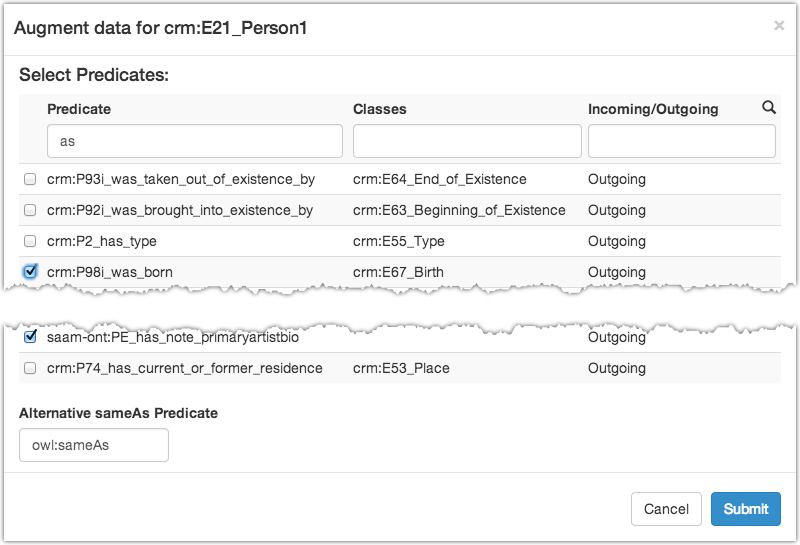
\includegraphics[width=4.9in]{images/5-search.png}
\vspace{-5mm}
\caption{A Karma user selects CIDOC CRM object and data properties discovered from other sources to augment crm:E21\_Person}
\vspace{-21pt}
\label{fig:search-screenshot}
\end{figure*}

\textbf{Step 3: Integrating Data Sources.} 
The user selects the artist's biography (for completeness) and birth (for validation). Karma then automatically constructs SPARQL queries for the data.
To facilitate the integration for this demo, we generated owl:sameAs links between the datasets' artists using LIMES \cite{ngomo2011limes}.  In future work we will investigate adding this process for the user.
Karma then merges the results and updates the source model appropriately as illustrated in Figure~\ref{fig:augment-screenshot}, so the user can continue to explore the integrated data interactively. 

\begin{figure*}
\begin{center}
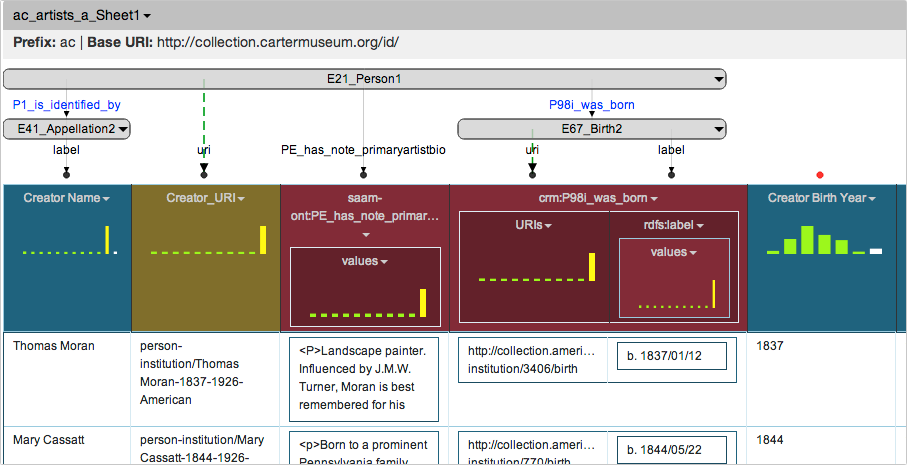
\includegraphics[width=4.9in]{images/6-augment.png}
\vspace{-3mm}
\caption{A Karma user has integrated biographical data from the Smithsonian into their dataset}
\vspace{-2mm}
\label{fig:augment-screenshot}
\end{center}
\vspace{-1.5em}
\end{figure*}

\section{Related Work and Conclusions} 
We see similarities in our approach with those used in relational database integration and semantic service composition.  
ORCHESTRA\cite{ives2008orchestra} starts, like \rtworml, by aligning database tables to a schema graph.  
For integration, heuristics are used to translate keyword searches over the graph into join paths using its Q query system. 
However, these joins are not guaranteed to be semantically meaningful, unlike the integration paths \karma finds using \rtworml.

Platforms such as iServe\cite{pedrinaci2010iserve} aim to capture Linked Services and make them discoverable and queryable by annotating them with their Minimal Service Model using an editor.
We have also repurposed \rtworml to capture service descriptions in Karma\cite{taheriyan12:lapis}, which means we can also enable our users to compose such services with other data sources. 


By building on \karma's ability to quickly model many source types, we demonstrate how museum curators can identify other linked museum data sources, identify relevant, available biographical attributes for their artists, link their artists to those other sources, and then integrate the data from those sources into their own dataset. 
Through this source discovery and integration, the museum curator can transparently compose and join other museums' sources and services in a semantically meaningful, interactive way not previously possible.
\vspace{-1mm}
\bibliographystyle{acm}
\bibliography{refs}
\end{document}